\documentclass{classrep}
\usepackage[utf8]{inputenc}

\usepackage{listings}
\usepackage{graphicx}
\usepackage[none]{hyphenat}
\usepackage{float}
\usepackage{geometry}
\usepackage{lipsum}
\usepackage{afterpage}

\studycycle{Informatyka, studia niestacjonarne}

\coursesemester{V}

\coursename{Sztuczna inteligencja i systemy ekspertowe}
\courseyear{2018/2019}

\courseteacher{dr inż. Przemysław Nowak}
\coursegroup{niedziela, 17:15}

\author{
  \studentinfo{Marcin Pajkowski}{211968} \and
  \studentinfo{Rafał Warda}{214067}
}

\title{Przeszukiwanie przestrzeni stanów}

\begin{document}

\begin{titlepage}
  \maketitle
  \thispagestyle{empty}
\end{titlepage}

\section{Cel}

Implementacja grafowych algorytmów przeszukiwania przestrzeni stanów;
porównanie metod ślepych i heurystycznych na przykładzie układanki
``piętnastka''.

\section{Wprowadzenie}

\subsection{O grze ``piętnastka''}

``Piętnastka'' jest grą z serii łamigłówek logicznych. W klasycznym wydaniu
jest zbudowana jako ramka, wewnątrz której znajdują się klocki. Jedno pole
tej konstrukcji zawsze jest wolne, umożliwia to graczowi przesuwanie klocków.
Celem rozgrywki jest ułożenie klocków w określonej kolejności - może to być
ciąg liczb naturalnych lub obrazek.

\subsection{Złożoność problemu i rozwiązywalność}

Nie wszystkie układy są rozwiązywalne. Możemy je podzielić na parzyste i nieparzyste - co
oznacza, że do uzyskania stanu wzorcowego należy wykonać parzystą lub
nieparzystą liczbę ruchów. Wszystkie układy powstające wskutek legalnego
przesuwania klocków - wykonując pierwszy ruch począwszy od układu docelowego - są układami parzystymi.
 Ilość stanów każdej układanki można wyznaczyć za pomocą wzoru:
$ iloscStanow = \frac{iloscPol!}2 $.

\subsection{Grafowa reprezentacja przestrzeni stanów}

Grafem nazywamy obiekt matematyczny składający się z niepustego zbioru
wierzchołków W i zbioru krawędzi K łączącego niektóre z tych
wierzchołków {[}1{]}. Graf może świetnie posłużyć do zapisu przebiegu
gry ``piętnastka''. Za wierzchołki grafu można przyjąć kolejne stany
planszy układanki, a krawędzie można zdefiniować jako kierunek
przesunięcia wolnego pola (tj. zamiany wolnego pola z elementem
znajdującym się względem niego nad nim, pod nim, z jego lewej lub prawej
strony).

\subsection{Metody przeszukiwania przestrzeni stanów}
\subsubsection{Podział algorytmów}
\begin{itemize}
  \item Metody ślepe (klasyczne):
    \begin{itemize}
      \item breadth-first search (BFS)
      \item depth-first search (DFS)
    \end{itemize}
  \item Metody oparte o heurystyki:
    \begin{itemize}
      \item algorytm A*
    \end{itemize}
\end{itemize}

Algorytmy klasyczne jako dodatkowy parametr przyjmują \emph{porządek
przeszukiwania}, zaś algorytm A* do przyspieszenia procesu
przeszukiwania wykorzystuje \emph{metryki} - zostaną zaprezentowane
metryka Hamminga oraz Manhattan (innymi nazwami tej metryki spotykane
w literaturze metryka taksówkowa lub metryka miejska).

\subsubsection{Breadth-First Search}

Algorytm BFS przeszukuje graf \emph{wszerz} - na początku
odwiedzany jest stan początkowy, następnie jego sąsiedzi
a w dalszej kolejności sąsiedzi sąsiadów rozwiniętych w poprzednich
iteracjach - do momentu znalezienia stanu wzorcowego.

\subsubsection{Depth-First Search}
Inaczej działa algorytm DFS: w literaturze można spotkać się ze
stwierdzeniem, że przeszukuje on graf \emph{w głąb}. Można łatwo to
uzasadnić - DFS po rozwinięciu stanu wyjściowego nie próbuje rozwijać stanów
na tej samej wysokości jak ma to miejsce W DFS. Zamiast tego odwiedza
stany-dzieci i rozwija je do momentu napotkanej przeszkody. Taką przeszkodą może
być koniec ścieżki w głąb (w wypadku układanki - brak możliwości przesunięcia
klocka w danym kierunku) lub arbitralnie ustalony limit osiąganej głębokości.

\subsubsection{A*}
Algorytm \emph{A*} przyjmuje inną strategię działania niż metody
omówione wyżej - nie opiera się na ściśle określonym porządku. Suplementem tego
algorytmu wspomagającym ustalenie dalszej kolejności przeszukiwania jest heurystyka.
Zostaną zaprezentowane dwie heurystyki - metryka Hamminga i Manhattan.
Stany oczekujące na przetworzenie odkładane są do listy, która jest uporządkowana
rosnąco według funkcji $ f(x) = g(x) + h(x) $, gdzie $ g(x) $ to długość ścieżki
od stanu wyjściowego do stanu $ x $, a $ h(x) $ oznacza aproksymowana odległość
do stanu docelowego według heurystyki $ h $.

\section{Implementacja}
\subsection{Stos technologiczny}

Program został napisany w technologii C++ 17 z wykorzystaniem biblioteki
Google Test wspierającej testy jednostkowe. Stan układanki przedstawiony
jest jako klasa State. Klasa ta zawiera jednowymiarową tablicę o
wielkości NxM - układanka została zrzutowana na jeden wymiar celem
zredukowania zjawiska \emph{cache miss}. Informacje o rzeczywystych
wymiarach zapisane są w atrybutach klasy. Do zrealizowania
poszczególnych metod przeszukiwania przestrzeni stanów posłużono się
algorytmami i strukturami danych dostępnymi w bibliotece STL języka C++.

\subsection{Usprawnienie DFS}

W przypadku ``czystego'' algorytmu DFS niemożliwe było znalezienie rozwiązań
układanki z arbitralnie ustawionym maksymalnym stopniu rekursji na 20. W tym celu zastosowano
pewną modyfikację algorytmu - jeżeli stan rozwijany lub odwiedzany znajduje się bliżej
stanu wyjściowego to stan ten będzie brany pod uwagę.

\section{Materiały i metody}
Do zrealizowania zadania zostały użyte następujące programy i skrypty wspomagające dostarczone razem z kartą
przedmiotu:
\begin{enumerate}
  \item Generator układanek,
  \item Walidator układanek,
  \item Wizualizator układanek,
  \item Skrypt uruchamiające program przeszukujący w trybie wsadowym (powłoka bash),
  \item Skrypt ekstraktujący dane wygenerowane podczas przeszukiwania (powłoka bash).
\end{enumerate}
Do stworzenia pliku binarnego programu generującego rozwiązania z kodu źródłowego C++ użyto kompilatora
Clang z pakietu LLVM. Wykresy zostały przygotowane w narzędziu Jupyter Notebook (kernel Python 3).
Użyto bibliotek pandas, numpy i matplotlib.

Algorytmy przeszukiwania przestrzeni stanów zostały porównane na podstawie parametrów takich jak:
\begin{itemize}
  \item długość ścieżki,
  \item ilość odwiedzonych stanów,
  \item ilość przetworzonych stanów,
  \item maksymalny stopień rekursji,
  \item czas przetwarzania algorytmu.
\end{itemize}

\section{Wyniki}

Wyniki zostaną zaprezentowane w następującej kolejności:
\begin{enumerate}
  \item Porównanie wszystkich algorytmów
  \item Wpływ wybranego porządku przeszukiwania dla algorytmów ślepych
    \begin{itemize}
      \item BFS
      \item DFS
    \end{itemize}
  \item Wpływ wybranej metryki dla algorytmu A*
\end{enumerate}

% All algorithms
\newgeometry{left=0.5cm,right=1cm,top=1.5cm, bottom=3cm}
\begin{figure}[H]
  \centering
  \makebox[\textwidth][c]{%
    \begin{minipage}{0.45\textwidth}
      \centering
      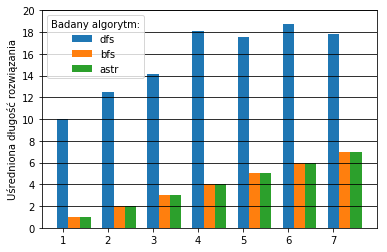
\includegraphics[width=1.1\textwidth]{output_3_0.png}
    \end{minipage}\hfill
    \begin{minipage}{0.45\textwidth}
      \centering
      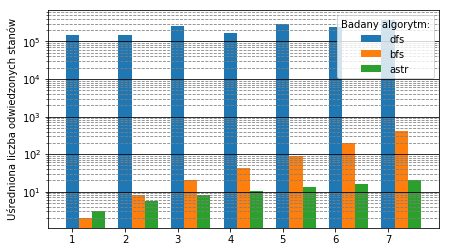
\includegraphics[width=1.1\textwidth]{output_3_1.png}
    \end{minipage}
  }%
\end{figure}
\begin{figure}[H]
  \centering
  \makebox[\textwidth][c]{%
    \begin{minipage}{0.45\textwidth}
      \centering
      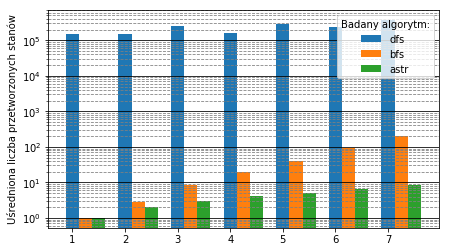
\includegraphics[width=1.1\textwidth]{output_3_2.png}
    \end{minipage}\hfill
    \begin{minipage}{0.45\textwidth}
      \centering
      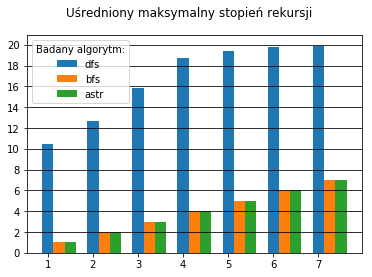
\includegraphics[width=1.1\textwidth]{output_3_3.png}
    \end{minipage}
  }%
\end{figure}
\begin{figure}[H]
  \centering
  \begin{minipage}{0.45\textwidth}
    \centering
    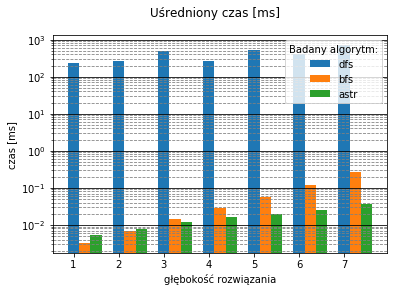
\includegraphics[width=1.1\textwidth]{output_3_4.png}
  \end{minipage}
\end{figure}

%end all algorithms

%bfs comp
\afterpage{
  \thispagestyle{empty}
  \begin{figure}[H]
    \centering
    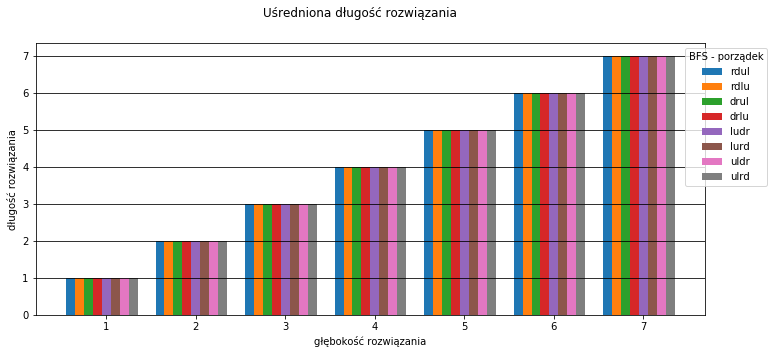
\includegraphics[scale=0.735]{output_5_0.png}
    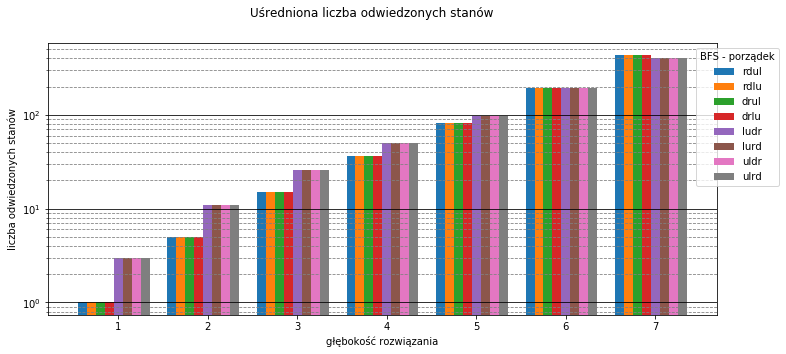
\includegraphics[scale=0.735]{output_5_1.png}
    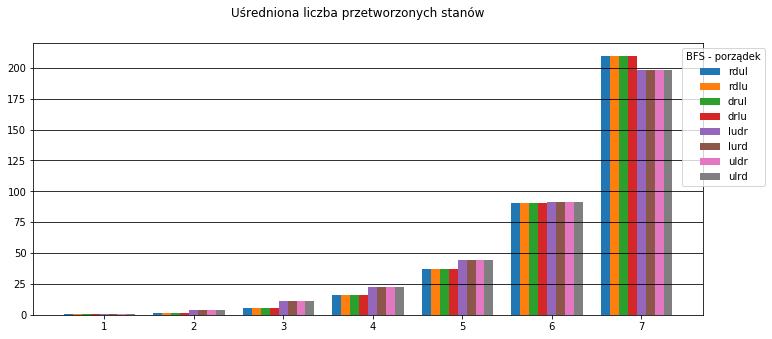
\includegraphics[scale=0.735]{output_5_2.png}
  \end{figure}
}
\begin{figure}[H]
  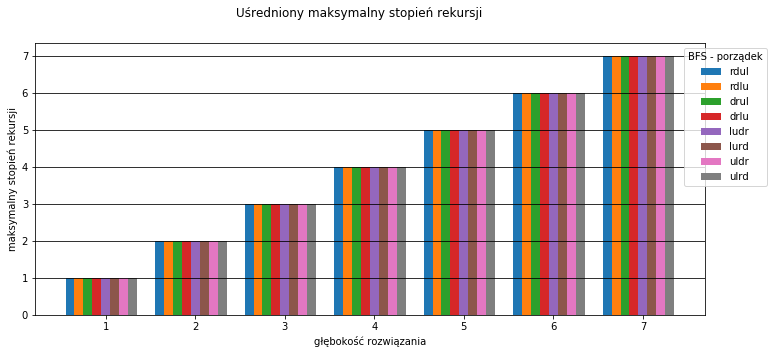
\includegraphics[scale=0.735]{output_5_3.png}
  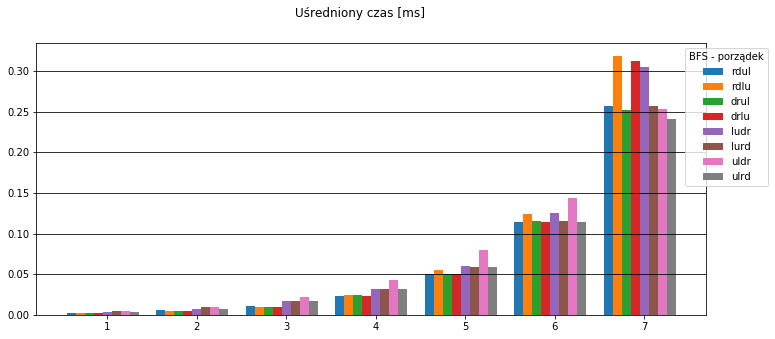
\includegraphics[scale=0.735]{output_5_4.png}
\end{figure}
%end bfs comp

%dfs comp
\afterpage{
  \thispagestyle{empty}
  \begin{figure}[H]
    \centering
    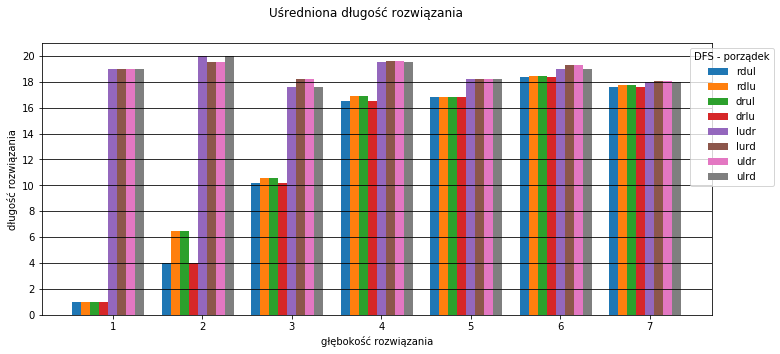
\includegraphics[scale=0.735]{output_6_0.png}
    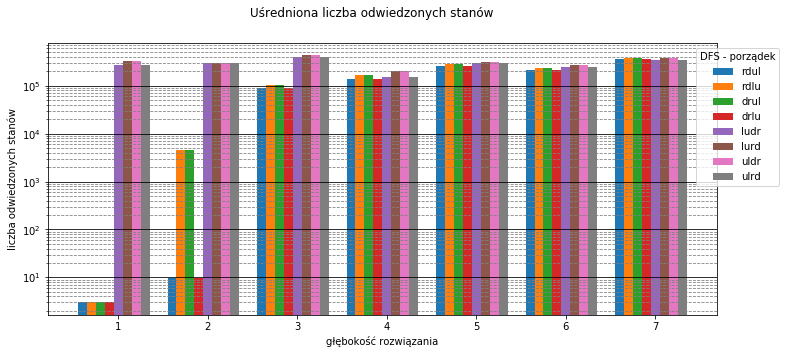
\includegraphics[scale=0.735]{output_6_1.png}
    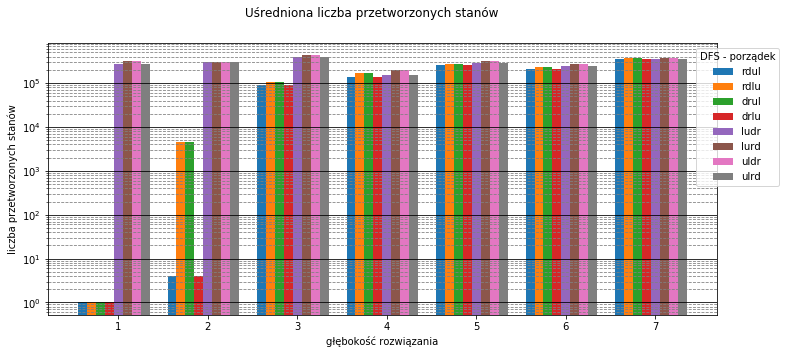
\includegraphics[scale=0.735]{output_6_2.png}
  \end{figure}
}
\begin{figure}[H]
  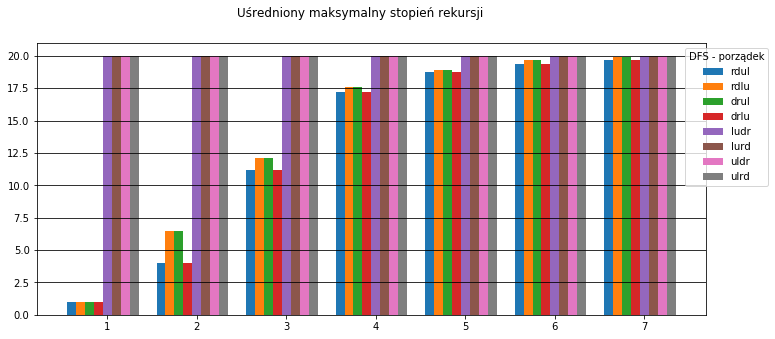
\includegraphics[scale=0.735]{output_6_3.png}
  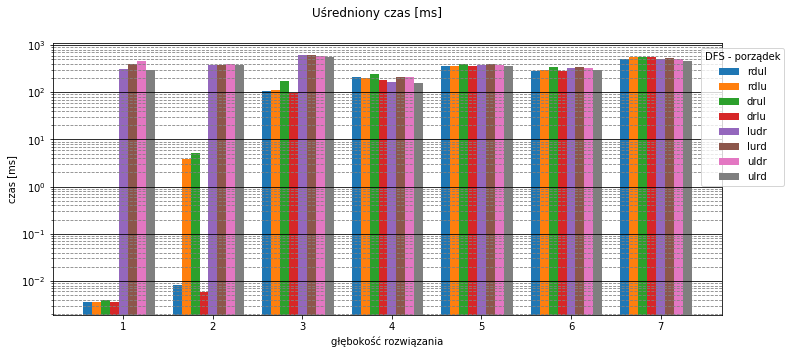
\includegraphics[scale=0.735]{output_6_4.png}
\end{figure}
%end dfs comp

%astr metrics comp
\begin{figure}[H]
  \centering
  \makebox[\textwidth][c]{%
    \begin{minipage}{0.45\textwidth}
      \centering
      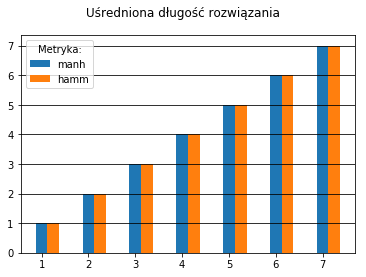
\includegraphics[width=1.1\textwidth]{output_4_0.png}
    \end{minipage}\hfill
    \begin{minipage}{0.45\textwidth}
      \centering
      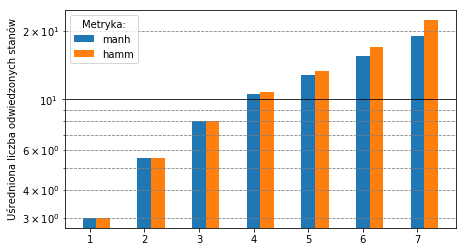
\includegraphics[width=1.1\textwidth]{output_4_1.png}
    \end{minipage}
  }%
\end{figure}
\begin{figure}[H]
  \centering
  \makebox[\textwidth][c]{%
    \begin{minipage}{0.45\textwidth}
      \centering
      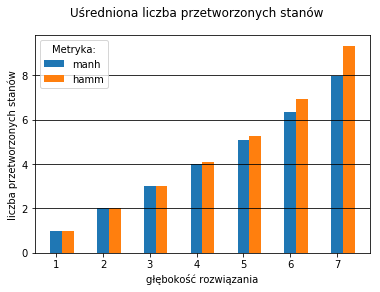
\includegraphics[width=1.1\textwidth]{output_4_2.png}
    \end{minipage}\hfill
    \begin{minipage}{0.45\textwidth}
      \centering
      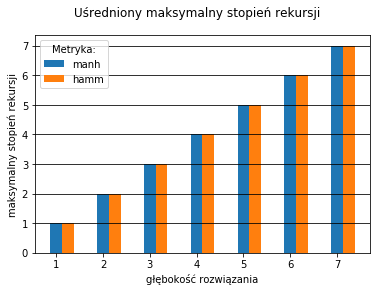
\includegraphics[width=1.1\textwidth]{output_4_3.png}
    \end{minipage}
  }%
\end{figure}
\begin{figure}[H]
  \centering
  \begin{minipage}{0.45\textwidth}
    \centering
    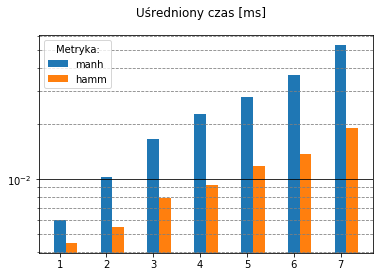
\includegraphics[width=1.1\textwidth]{output_4_4.png}
  \end{minipage}
\end{figure}
%end astr metrics comp

\restoregeometry

\section{Dyskusja}
\subsection{Optymalność badanych algorytmów}

Spośród testowanych algorytmów BFS i A* znajdowały zawsze rozwiązanie optymalne. W wypadku DFS w ogólności nie
jest to prawdą. BFS sprawdza najpierw wszystkie stany znajdujące się w takiej samej odległości od stanu
wyjściowego. Dzięki takiej taktyce odtworzenie ścieżki zawsze da optymalny wynik. Dla porównania, droga
tworzona przez DFS jest zupełnie inna - algorytm dopóki nie napotka przeszkody (w wypadku układanki - np. brak
możliwego ruchu w danym kierunku) będzie wchodził wgłąb grafu, przez co rozwiązania znajdujące się naprawdę
blisko mogą zostać przeoczone.

Algorytm A* jest zawsze optymalny przy założeniu, że użyliśmy prawidłowej heurystyki, tzn takiej która nie
przeszacowuje faktycznego kosztu.

\subsection{Ilość przetwarzanych danych}

DFS po raz kolejny wyróżnia się pośród badanych algorytmów - przetwarza zdecydowanie najwięcej stanów.
Najlepiej w tym zestawieniu wypada algorytm A*, w szczególności z metryką Manhattan - można to zauważyć
zwłaszcza dla głębokości większej niż 5.

\subsection{Szybkość działania}

Dla głębokości rzędów 1 i 2 BFS wypada nieznacznie lepiej, jednakże tendencja ta zaczyna się odwracać już w
momencie, gdy szukamy rozwiązań układanek o głębokościach większych lub równych 3. Co ciekawe, W zestawieniu
średnich czasów dla metryk Manhattan zostaje daleko w tyle za metryką Hamminga i ten trend wydaje się być
rosnący. Te dwa spostrzeżenia - BFS szybszy dla głębokości mniejszej niż 3 oraz A* z metryką Hamminga szybsza
niż A* z metryką Manhattan - mają wspólne wyjaśnienie. Przy małej głębokości układanki duże znaczenie ma koszt
umieszczenia stanu na liście frontier. W implementacji stworzonej na potrzeby zadania  dla BFS koszt
ten jest równy kosztowi wstawienia elementu do kolekcji. W wypadku algorytmu A* koszt wstawienia jest
dodatkowo powiększony o obliczenia związane z zastosowaną metryką, przy czym obliczenie odległości Hamminga
jest znacznie tańsze niż obliczenie odległości taksówkowej. Aby dać możliwość głosu obrony metryki Manhattan w
znajdowaniu najkrótszej drogi w grafie przeprowadzono dodatkowe badanie na układance o głębokości 20. W tej
próbie odnotowano następujące czasy:

\begin{itemize}
  \item Manhattan: 59.688 ms.
  \item Hamming: 581.177 ms.
\end{itemize}

Jest to niestety wyłącznie jedna próbka, zatem nie można na jej podstawie udowodnić tezy, że metryka Manhattan
dla dużych głębokości pozwala znaleźć rozwiązanie szybciej niż metryka Hamminga, jednakże na pewno zachęca do
przeprowadzenia dalszych badań na układankach o głębokościach większych niż 7.

Na temat szybkości algorytmu DFS można powiedzieć niestety tyle, że w ogólności odstaje ona od czasów
wykonania algorytmów BFS i A*. Dobre rezultaty można zaobserwować jedynie w wypadkach korzystnych szeregów
przeszukiwania.

\section{Wnioski}
\begin{itemize}
  \item BFS i A* to algorytmy zupełne i optymalne,
  \item Nie należy stosować DFS do przeszukiwania grafu przestrzeni stanów,
  \item Zastosowanie przeszukiwania heurystycznego znacznie redukuje liczbę odwiedzonych i przetworzonych
    stanów.
\end{itemize}

\begin{thebibliography}{0}
  \bibitem{l2short}
  \textsl{http://theory.stanford.edu/\textasciitilde{}amitp/GameProgramming/Heuristics.html}
  \bibitem{l2short}
  \textsl{http://wms.mat.agh.edu.pl/\textasciitilde{}zankomar/wyklady/Wyklad8.htm}
  \bibitem{l2short}
  \textsl{https://pandas.pydata.org/pandas-docs/stable/comparison\textunderscore{}with\textunderscore{}sql.html}
\end{thebibliography}

\end{document}

